\documentclass[25pt, a0paper, portrait, margin=0mm, innermargin=15mm,blockverticalspace=15mm, colspace=15mm, subcolspace=8mm, ngerman]{tikzposter}

\usepackage[utf8]{inputenc}
\renewcommand{\refname}{References}
\usepackage{lipsum} 
\usepackage{fancyhdr}
\usepackage[scaled]{helvet}
\renewcommand\familydefault{\sfdefault} 
\usepackage[T1]{fontenc}
\usepackage{transparent} % Transparent imanges

\usepackage{soulutf8} % Marking texts
%\sethlcolor{} % Color for marking texts

\usepackage[backend=biber,
    style=numeric-comp,
    maxcitenames=1,
    maxbibnames=1,
    %backref=true
    ]{biblatex}

\usepackage{colortbl} % Colored tables
\usepackage{xspace}

\usepackage{tikz}
\usetikzlibrary{arrows,shapes}

\usepackage{enumitem} % change the points of itemization

% selbst hinzugefügte Pakete
\usepackage{url}

\tikzposterlatexaffectionproofoff % 
\usetheme{Simple} %

% ---- Colors
\definecolor{mypink1}{rgb}{0.858, 0.188, 0.478}
\definecolor{titlecolor}{RGB}{74, 114, 159}
\definecolor{titledarkcolor}{RGB}{51,102,153}
\definecolor{LightGrey}{RGB}{232, 232, 232}
\definecolor{Grey}{RGB}{222, 223, 225}
\definecolor{DarkerGrey}{RGB}{215,217,219}
\definecolor{FontColor}{RGB}{131,136,138}
\definecolor{Red}{RGB}{204,0,0}
\definecolor{L-lig}{RGB}{25,124,192}
\definecolor{point-lig}{RGB}{54,104,163}
\definecolor{G-lig}{RGB}{62,66,68}

\definecolor{title-background}{RGB}{255,255,255}
\definecolor{title-foreground}{RGB}{0,0,0}


\definecolor{Orange}{RGB}{240,163,10} 
\definecolor{Gray}{RGB}{186,200,211}
\definecolor{LightRed}{RGB}{214,98,93}
\definecolor{LightBlue}{RGB}{160,200,217}
\definecolor{LightGreen}{RGB}{130,161,119}
\definecolor{Violet}{RGB}{190,144,252}
% ----

\colorlet{blocktitlefgcolor}{point-lig} % Title of blocks
\colorlet{blocktitlebgcolor}{Grey} % Lines for blocks
%\colorlet{blockbodybgcolor}{mypink1}%????
\colorlet{blockbodyfgcolor}{FontColor} % Textcolor within a block
%\colorlet{innerblocktitlebgcolor}{G-lig}
\colorlet{innerblocktitlebgcolor}{L-lig}
\colorlet{innerblocktitlefgcolor}{white}

% Notes
\colorlet{notefrcolor}{Red!60} % Color of notes
\colorlet{notefgcolor}{white} % Color of note test
\colorlet{notebgcolor}{Red!60} % Color of note background


% ---- Title
\settitle{ 
    \begin{minipage}{0.2\linewidth}
        \vspace{-15cm}
        %%% insert second logo at the top
        %\transparent{0.6}
\includegraphics[scale=1.1]{images/Logos/logoMIAI_white.png}
        \vspace{8.0cm}     
        \hspace{2.2cm}\transparent{1.0}
\includegraphics[scale=1.0]{images/Logos/HSEL_Allgemeines_Logo.eps}                

    \end{minipage}
    \hspace{6cm}
    \begin{minipage}[b]{0.8\linewidth}
        \vspace{2.0cm}
        \hspace{0cm}\color{title-foreground}{\Huge\textsc{\textbf{\@title}} \par } \vspace*{1em} \hspace{0cm}\color{title-foreground}{\Large \@author \par} \vspace*{1em} \hspace{0cm}{\@institute}\vspace{0.5cm} 
    \end{minipage}
}

\definetitlestyle{sampletitle}{
width=840mm, roundedcorners=0, linewidth=2pt, innersep=15pt,
titletotopverticalspace=0mm, titletoblockverticalspace=30mm
}{\begin{scope}[line width=\titlelinewidth, rounded corners=\titleroundedcorners]\draw[fill=title-background, color=title-background]
(\titleposleft,\titleposbottom) rectangle (\titleposright,\titlepostop);
\end{scope}}



\title{\parbox{1700pt}{Studienarbeit Virtual Reality: Remote Steuerung}}

\author{Christian Kitte, Prof. Dr. Thies Pfeiffer}
\institute{University of Applied Sciences Emden/Leer, Faculty of Technology, Department of Electrical Engineering and Informatics}

\usetitlestyle[]{sampletitle}
\setlength{\columnseprule}{0.4pt}
\addbibresource{Biblio/Biblio.bib}

%%%%%%%%%%%%%%%%%%%%%%%%%%%%%%%%%%%%%%%%%%%%%%%%%%%%%%%%%%%
\begin{document}
\maketitle

% --- Lines between the columns
\draw[DarkerGrey, line width=2mm, loosely dotted] (-13,35) -- (-13,-45); 
\draw[DarkerGrey, line width=2mm, loosely dotted] (15,35) -- (15,-45);

%------------------------------------------------------------------------------
% --------------------- Main body of the poster           ---------------------
\begin{columns}
\column{1}
\begin{subcolumns}

    %%%%%%%%%%%% COLUMN 01 %%%%%%%%%%%%%
    \subcolumn{.33}
   
    % --------------------------------- INTRODUCTION ----------
        \block{\textsc{Technische Einordnung}}{
            \begin{itemize}
                \item {\bf Technik:} Interaktion/ Visualisierung
                \item {\bf Geräte:} HMD Head Set/ XR Controller
                \item {\bf Interaktionstechnik:} Ray Casting/ Thumbstick zur Selektion/ Transformation/ Rotation
                \item {\bf Herausforderung:} Feedback/ Mapping/ Präzision/ Steuerung aus der Ferne 
            \end{itemize} \vspace{-2cm}
        
        }

    % --------------------------------- SECTION 01 ----------
        \block{\textsc{Aufgabenstellung}}
        {
            Innerhalb einer Virtuellen Umgebung (VR) sollen einzelne Objekte einer Gruppe über einen Zeitraum permanent selektiert und neu positioniert werden können.
            
            \vspace{1em}
            
            Selektion, Bewegung und das Ablegen sollen hierbei auch aus der Ferne (Remote) präzise und ohne direkte Sicht auf das ausgewählte Objekt möglich sein.
            
            \vspace{-2cm}
        }
        
      % --------------------------------- SECTION 02  ----------    
        \block{\textsc{Technische Herausforderung}}
        {
           Als besondere Herausforderungen können vor allem die folgenden vier Punkte identifiziert werden:
            
            \vspace{1em}
            
            \begin{itemize}
                
                \item Ein Gruppenkonstrukt, welches sich aus geeigneten, intrinsischen Merkmalen eines Objektes herleitet und dieses eindeutig einer Gruppe zuordnet.
                
                \item Ein Mechanismus zum Erkennen und zur Selektion von Objekten anhand definierter, intrinsischer (Gruppen)Merkmale.
          
                \item Ein Interaktionskonzept, um Objekte präzise und sicher aus der Ferne navigieren zu können. Dies umfasst sowohl die Transformation als auch die Rotation.

                \item Ein Feedbacksystem, welches einen eindeutigen und präzisen Rückschluss auf den Zustand und die Position eines Objektes zulässt.

            \end{itemize}
            
            \vspace{-2cm}
        }
          
        \block{\textsc{Lösungsansatz}}
        {
            Der hier vorgestellte, prototypische Lösungsansatz basiert auf der Entwicklungsumgebung Unity \cite{Unity} in der Version 2020.3.25 LTS. Für die Interaktion kam Oculus Quest (HMD) unter Anwendung des freien und quelloffenen Standards OpenXR \cite{Khronos} in der Version 1.3.1 zum Einsatz.
            
            \vspace{1em}

            Konzeptionell handelt es sich um ein erweitertes XR Rig. Ein XR Rig ist eine Softwarekomponente, welche die Logik für alle Interaktionen und Sinneswahrnehmungen des Spielers mit der VR beinhaltet. Sie wirkt als Mittler zwischen dem HMD und seinen Controllern auf der einen, der VR auf der anderen Seite.
        
            \vspace{1em}
            
            Je ein Controller ist für den Teilaspekte Steuerung eines Objektes (links) sowie Steuerung des Charakters (rechts) zuständig. Während das Mapping und die Interaktion des rechten Controllers der von Unity vorgestellten Musterlösung folgen, verfügt der linke Controller über ein eigenständiges Interaktionskonzept mit angepassten Mapping.

            \vspace{1em}

            Zur Selektion wird ein modifiziertes Ray Casting \cite{Raycast} eingesetzt, welches nur die Interaktion mit bestimmten Objekten zulässt und über die Triggertaste aktiviert wird. 

            \vspace{-2cm}
        }
        
    %%%%%%%%%%%%%%% COLUMN 02 %%%%%%%%%%%%%
    \subcolumn{.33}
    
    % --------------------------------- SECTION 03  ----------
        \block{\textsc{Lösungsansatz}}
        {
            Über die Griptaste kann ein erfasstes Objekt permanent selektiert werden. Dies ermöglicht die Transformation und Rotation mit Hilfe des Thumbsticks innerhalb der VR. Bezugssystem ist das globale Koordinatensystem.
            
            \vspace{1em}
            
            Die Gruppierung selektierbarer Objekte erfolgt durch eine Annotation mit Hilfe der Tag Eigenschaft, über welches jedes Unity Game Object verfügt. Weitere Modifikationen sind nicht erforderlich.
            
            \vspace{1em}
            
            Bei einer Selektion wird anhand zweier verschiedenfarbiger Pfeile eine Vorwärts- (Weiß, globale Z-Achse) und Rechtsbewegung (Grün, globale X-Achse) permanent visualisiert (Abb. 1). Die Ausrichtung passt sich dynamisch der Blickrichtung des Spielers an.
            
            \vspace{1em}
            
            Zusätzlich wird eine permanente, visuelle Rückmeldung (Informationssystem) dargestellt und im Blickfeld des Charakters angezeigt (Abb. 1). Dieses Umfasst:
            
             \begin{itemize}
             
                \item eine Textanzeige mit dem Namen und der Höhe des aktuell selektierten Objektes. 
                \item drei Kamera Aufnahmen des selektierten Objekts von oben, hinten und rechts relativ zum oben genannten Bezugssystem. 
                \item ein eingeblendetes Lot zum Untergrund, wenn eine definierte Höhe unterschritten wird.
            
            \end{itemize}
            
            \vspace{1em}
            
            \innerblock{Informationssystem}{
                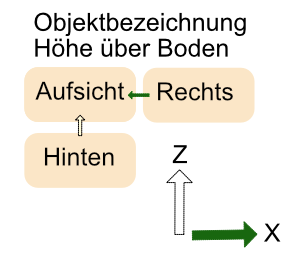
\includegraphics[scale=1.5]{images/uebersicht.png}
                \label{Informationssystem:Informationssystem}
                \newline
	            \caption{Abbildung 1 - Verdeutlichung des eingeblendeten Informationssystems. Die kleinen Pfeile geben die Blickrichtung relativ zu den globalen Achsen Z und X an.}
	        }
	        
            \vspace{-2cm}
        }
        
    % --------------------------------- SECTION 04  ----------
        \block{\textsc{Anwendungsbeispiel}}
        {
            Zur Evaluation der Lösung wurde unter Verwendung von Unity ein Anwendungsszenario mit einer konkreten Aufgabenstellung entwickelt.
            
            \vspace{1em}
            
            Das Szenario stellt sich als durch eine Vertiefung (Schlucht) geteilte Ebene dar. Ein Überwinden ohne Hilfe ist hierbei nicht möglich.
            
            \vspace{1em}
            
            Innerhalb der Schlucht existieren Pfeiler unterschiedlicher Höhe. Auf der Seite des Spielers (Startseite) befinden sich Stege. Ziel ist das Erreichen der anderen Seite (Zielseite).
            
            \vspace{1em}
            
            Die Zielseite kann nur erreicht werden, indem mit den Stegen und unter Ausnutzung der Pfeiler ein Pfad über die Schlucht gebaut wird. Hierzu müssen die Stege zwischen Rand und Pfeiler, respektive Pfeiler und Pfeiler ablegen werden.
            
            \vspace{1em}
            
            Aufgrund der unterschiedlichen Höhen der Pfeiler können nur ungerade Pfade erstellt werden, welche von keiner Seite komplett einsehbar sind.
            
            \vspace{-5cm}
        }

  %%%%%%%%%%%%%%%%%%%%%%%% COLUMN 03 %%%%%%%%%%%%%%%%%%%%%%%%%   
    \subcolumn{.33}
    
    % ------------------------------------ SECTION 05  ------------
        \block{\textsc{Ergebnisse}}
        {
            Als Ergebnis konnte gezeigt werden, dass es mit dem hier vorgestellten Lösungsansatz möglich ist, aus der Ferne allein auf Basis der visuellen Rückmeldung ein Objekt präzise zu steuern und zu positionieren, auch wenn dessen konkrete Position nicht einsehbar ist.
            
            \vspace{-2cm}
        }
        
    % ---------------------------------------------
        \block{\textsc{Diskussion}}
        {
             Für Interaktionen in die Ferne existieren eine Reihe effizienter Möglichkeiten. Zu nennen sind hier Ray Casting oder GoGo \cite{Grabbing}. Sie alle benötigen jedoch einen freien Blick auf das Geschehen und fokussieren primär auf das Ergreifen. Als Referenz für eine naive Umsetzung wurde Ray Casting in der von Unity empfohlenen Weise \cite{Raycast} umgesetzt. 
            
            \vspace{1em}
            
            Hierbei wird mit Hilfe eines Strahls ein selektierbares Objekt fokussiert. Ändert der Strahl seine Farbe, kann das aktuell fokussierte Objekt durch Betätigung der Grip Taste am Controller "aufgehoben" werden. Im Vergleich ermöglicht die hier vorgestellte Lösung bei gleicher Technik ein deutlicheres Feedback, indem das jeweils aktive Objekt selbst hervorgehoben wird. Zudem ist der Strahl nur während der Auswahl sichtbar.
            
            \vspace{1em}
            
            Bei einer naiven Selektion verbleibt das selektierte Objekt je nach Konfiguration entweder an seiner Position oder wird zum Controller verschoben. In diesem Zustand kann es bis zur Freigabe durch Bewegung des Controllers bewegt und auf dem Strahl verschoben und rotiert werden. Im Gegenzug erfolgt bei der angepassten Lösung zunächst eine permanente Selektion. Anschließend kann eine Steuerung über den Thumbstick des linken Controllers erfolgen, jedoch auch beliebig pausiert werden. Die Vorteile dieser Technik bei der Bewegung (siehe  \cite{Locomotion}) werden auch für die Transformation und Rotation eines entfernten Objektes angenommen. Zudem wird die Bewegungsanweisung von der Eigenbewegung des Controllers entkoppelt. Der Charakter ist in seiner Handlung somit freier.
            
            \vspace{1em}
            
            Insbesondere in der Ferne zeigen sich bei der vorgestellten Lösung durch das Mitführen und der Verwendung separater Kameras mit konstanter Bildqualität Vorteile gegenüber der naiven Lösung. Hier kommt es mit zunehmender Entfernung zu starken Defiziten in der räumlichen Wahrnehmung sowie einem Zittern des Strahls. Eine genaue Positionierung wird erschwert und ist ab einer gewissen Entfernung unmöglich. Die erweiterte Lösung zeigt hier eine konstante Präzision der Steuerung. 
            
            \vspace{1em}
            
            Im direkten Vergleich, wurde die Aufgabe jeweils in etwa 12 Minuten gelöst. Hierbei kam es jedoch bei der naiven Umsetzung zu vier Fehlversuche. Mit dem vorgestellten Konzept war bereits der erste Versuch erfolgreich. 
            
            \vspace{1em}
            
            Subjektiv wurde das vorgestellte Konzept als zunehmend einfacher, das naive als zunehmend anstrengender in der Bedienung empfunden. 
        }

    % ----------------------------------------------
        \block{}{
        \vspace{-1cm}
            \textbf{AR}: Augmented Reality $\bullet$
            \textbf{HCI}: Human Computer Interaction $\bullet$
            \textbf{MR}: Mixed Reality $\bullet$  
            \textbf{VR}: Virtual Reality $\bullet$ 
            \textbf{XR}: Sammelbegriff für VR/ AR/ MR
        
        \vspace{1cm}
        
            \url{https://github.com/ChristianKitte/InteraktionskonzeptUnity}
        }

    \end{subcolumns}
    

    % ---------------------------------  BIBLIO  ----------
        \block{}{
            \vspace{-6cm}
            \printbibliography
        }
        
\end{columns}

% ----------------- Footer line -------------
\node [above right, text=white,outer sep=45pt,minimum width=\paperwidth, align=center, draw, fill=titledarkcolor, color=point-lig] at (-43.6,-61) {\textcolor{white}{\normalsize e-mail: christian.kitte@stud.hs-emden-leer.de $\bullet$ 
thies.pfeiffer@hs-emden-leer.de $\bullet$ 
www: https://www.mixality.de} };

\end{document}
